%%%%%%%%%%%%%%%%%%%%%%%%%%%%%%%%%%%%%%%%%%%%%%%%%%%%%%%%%%%%%%%%%%%%%%%%%%%%%%%%
% Author : [Name] [Surname], Tomas Polasek (template)
% Description : Seventh exercise in the Introduction to Game Development course.
%   It deals with the creation of a Game Design Document, presenting a short 
%   pitch for a potential game project.
%%%%%%%%%%%%%%%%%%%%%%%%%%%%%%%%%%%%%%%%%%%%%%%%%%%%%%%%%%%%%%%%%%%%%%%%%%%%%%%%

\documentclass[a4paper,10pt,english]{article}

\usepackage[left=2.50cm,right=2.50cm,top=1.50cm,bottom=2.50cm]{geometry}
\usepackage[utf8]{inputenc}

% Hyper-Text References
\usepackage{hyperref}
\hypersetup{colorlinks=true, urlcolor=blue}

% Drawing Images and Graphs
\usepackage{tikz}
\usepackage{pgfplots}

% Page Utilities
\usepackage{graphicx}

% Image Sub-Captions
\usepackage{subcaption}

\newcommand{\ph}[1]{\textit{[#1]}}

\title{%
Game Pitch Document%
}
\author{%
Antonín Masopust (xmasop05)%
}
\date{}

\begin{document}

\maketitle
\thispagestyle{empty}

{%
\large

\begin{itemize}

\item[] \textbf{Title:} Starlight

\item[] \textbf{Genre:} Platformer

\item[] \textbf{Style:} 2D / vector graphics

\item[] \textbf{Platform:} iOS/Android

\item[] \textbf{Market:} Casual gamers (mostly young)

\item[] \textbf{Elevator Pitch:} A blue fox running on different planets and looking for lost start.

\end{itemize}

}

\section*{\centering The Pitch}

\subsection*{Introduction}
Starlight is a 2D platformer about a fox (named Starlight), who is running through planets in search of lost stars from the Vulpecula constellation. Along the way, she encounters different obstacles and enemies, while also learning new abilities.

\subsection*{Story}
A powerful and ruthless wind soared through space and blew apart the Vulpecula constellation. All the stars were scattered across various planets. That's where our main character comes into play. Starlight - the spirit of the Vulpecula constellation - takes form of a blue fox and begins her search for the stars. She ventures the hostile planets in hope of restoring the former state of the constellation. During her search, she unexpectedly finds a bright pulsar adding it to her collection and making the constellation even better. At the end, when she finds all stars, she leaves her tangible state and continues her existence as the Vulpecula spirit.

\subsection*{Gameplay}
The game is a 2D platformer with the main character constantly running to the right. The game is divided into 5 worlds (planets) and there are multiple levels on each. Every planet has different obstacles (walls, trees, waters, ancient ruins) and enemies (wild animals, fictional creatures, robots). The player can overcome them with jumping, sliding, climbing and various attacks like bite, tail sweep or energy pulse, which will be unlocked during the playthrough.

\subsection*{Platform}
The game is meant for mobile devices (iOS, Android). This will reflect in controls, because the input will be from a touchscreen. It will be played in landscape mode and different actions will be performed by specific gestures e. g. swipe, tap, drawing a circle or hat.

\subsection*{Background}
The main inspiration for this game came from Vector – mobile, parkour runner and Ori and The Blind Forest – a platforemr with a spirit as the main character saving the forest.

\subsection*{Style}
Vector graphics toned to blue and purple colors.

\begin{figure}[ht]
    \centering
    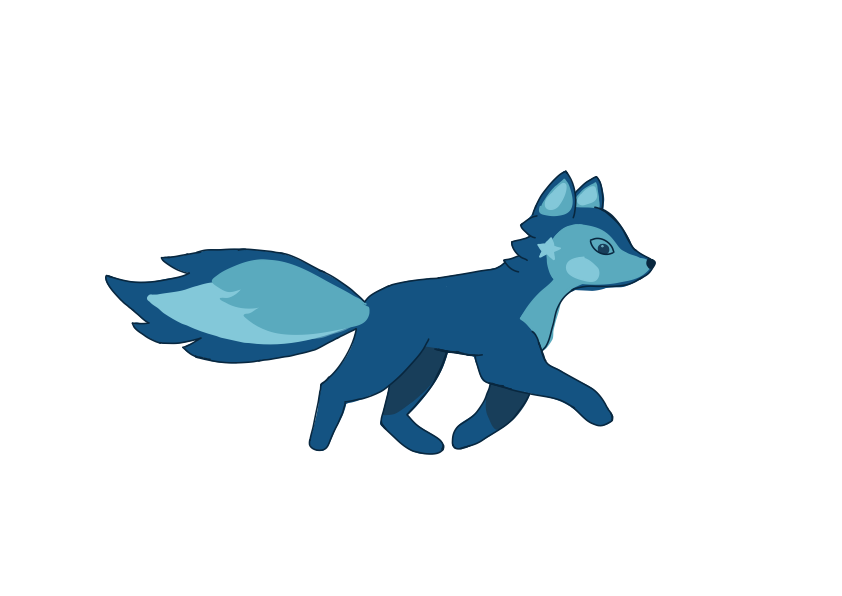
\includegraphics[width=0.7\linewidth]{starlight.png}
    \caption{Starlight}
\end{figure}
\begin{figure}[ht]
    \centering
    
\includegraphics[width=0.5\linewidth]{concept.png}
    \caption{Concept}
\end{figure}
\begin{figure}[ht]
    \centering
    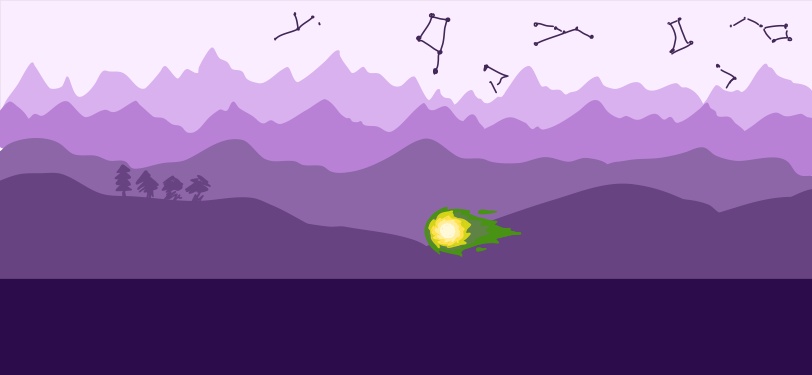
\includegraphics[width=0.7\linewidth]{background.png}
    \caption{Background}
\end{figure}

\end{document}